% !TEX root = ../main.tex
% Chapter 1 - Introduction
\chapter{Introduction} % Main chapter title
\label{Chapter1} % For referencing the chapter elsewhere, use \ref{Chapter1}

% Introduction ----------------------------------------------------------------------------------------
The awe--inspiring power of a starry night sky is something we might not experience too often these days thanks to light and atmospheric pollution.
Every once in a while on clear nights though, I find myself gazing at the sky, wondering about these flickering lights.
What are these mysterious, strange dots? Where do they come from? How did they get there?

Just an occupational predisposition of an astrophysicist? Maybe\dots~but these questions have been asked since people could tilt their heads back:
\vspace{3pt}
\begin{displayquote}
 \textit{\dots neque enim clipei caelamina novit,\\
 Oceanum et terras cumque alto sidera caelo\\
 Pleiadasque Hyadasque inmunemque aequoris Arcton\\
 diversosque orbes nitidumque Orionis ensem.}
\end{displayquote}
\begin{flushright} -- Ovid, Metamorphoses, liber xiii, 291--294 \end{flushright} \vspace{6pt}

This ancient, Latin poem--extract describes the fabled shield of the legendary hero of the Trojan war, Achilleus.
Loosely translated it says: 'For, he understands nothing of the shield's reliefs~\footnote{as in engravings}, of the ocean, the lands, and the starry sky high above, the Pleiades, the Hyades and the Bear, clear of the sea~\footnote{sometimes also translated as Milky Way}, and on the other side of the heavens Orion's sparkling sword.'

Orion was, as the myth goes, a master huntsman, so sure of his skills that he accompanied the gods on a hunt, only to be --- ironically --- stung by one of the smallest animals, the scorpion.
Nonetheless, Zeus must have been impressed by Orion, because he placed him among the stars to the opposite side of the Scorpio constellation.

This and numerous myths like it, tried to give an explanation for the origin of the strange view of the night sky and its constellations in the past.
Presently, the Orion constellation is one of the most studied regions in astronomy; see \citet{Orion_Survey} for a recent, comprehensive study of the whole Orion region performed with the Hubble Space Telescope.

% Orion ----------------------------------------------------------------------------------------
The Orion constellation is not only interesting for its considerable fraction of the brightest, most massive stars in our galaxy, but also because it harbors the Orion molecular cloud complex which is thought to be an extraordinarily active star forming region.
Molecular clouds, generally considered the birth places of stars, have very high densities compared to other regions in our galaxy.
From thorough studies we know that these loosely bound clouds form clumps in which the density reaches even higher values such that gravity wins over the opposing thermal pressure (and possibly other stabilizing effects) and their collapse to protostars is initiated.

Although stars are probably the best comprehended astronomical objects in the visible universe, their formation process is still quite puzzling.
The reason for it might be our clouded sight, and that quite literally.
An observation of star formation is problematic, because during the period of time preceding it, there is usually no sufficiently bright light source in order to be noticeable through the cloud's dense material; and even if shining stars were already formed there, they would most certainly be obscured by it.
However, advances in modern technology make observations of star formation, as well as our understanding of the physics behind it, gradually tangible.
\\[6pt]
%
In this thesis the discussion of the complicated subject of molecular clouds will only scratch the surface of knowledge acquired over the years.
Thus, for a broader overview on molecular clouds or a detailed discussion on any topic concerning star formation, I refer to the starting chapters of the very informative book of \citet{Stahler_Palla}.

% ----------------------------------------------------------------------------------------
\section{Molecular clouds observed}
\label{sec:MolecularClouds}
Considering the topic of this thesis, there is finally a valid reason to present pictures of these breathtaking, astronomical objects, so commonly used as desktop wallpapers.
The beauty of such spectacular views --- in an aesthetic, as well as scientific sense --- lies in their complexity and diversity.
Gravity, thermal pressure, turbulence, magnetic fields, radiation, chemical composition, and potentially a multitude of other influences are believed to be determining factors for processes to be found in molecular clouds.

% The picture ----------------------------------------------------------------------------------------
\figref{fig:Orion_nebula} shows a composite image in the infrared and visible spectra of the Orion nebula.

\begin{figure}[ht]
 \centering
 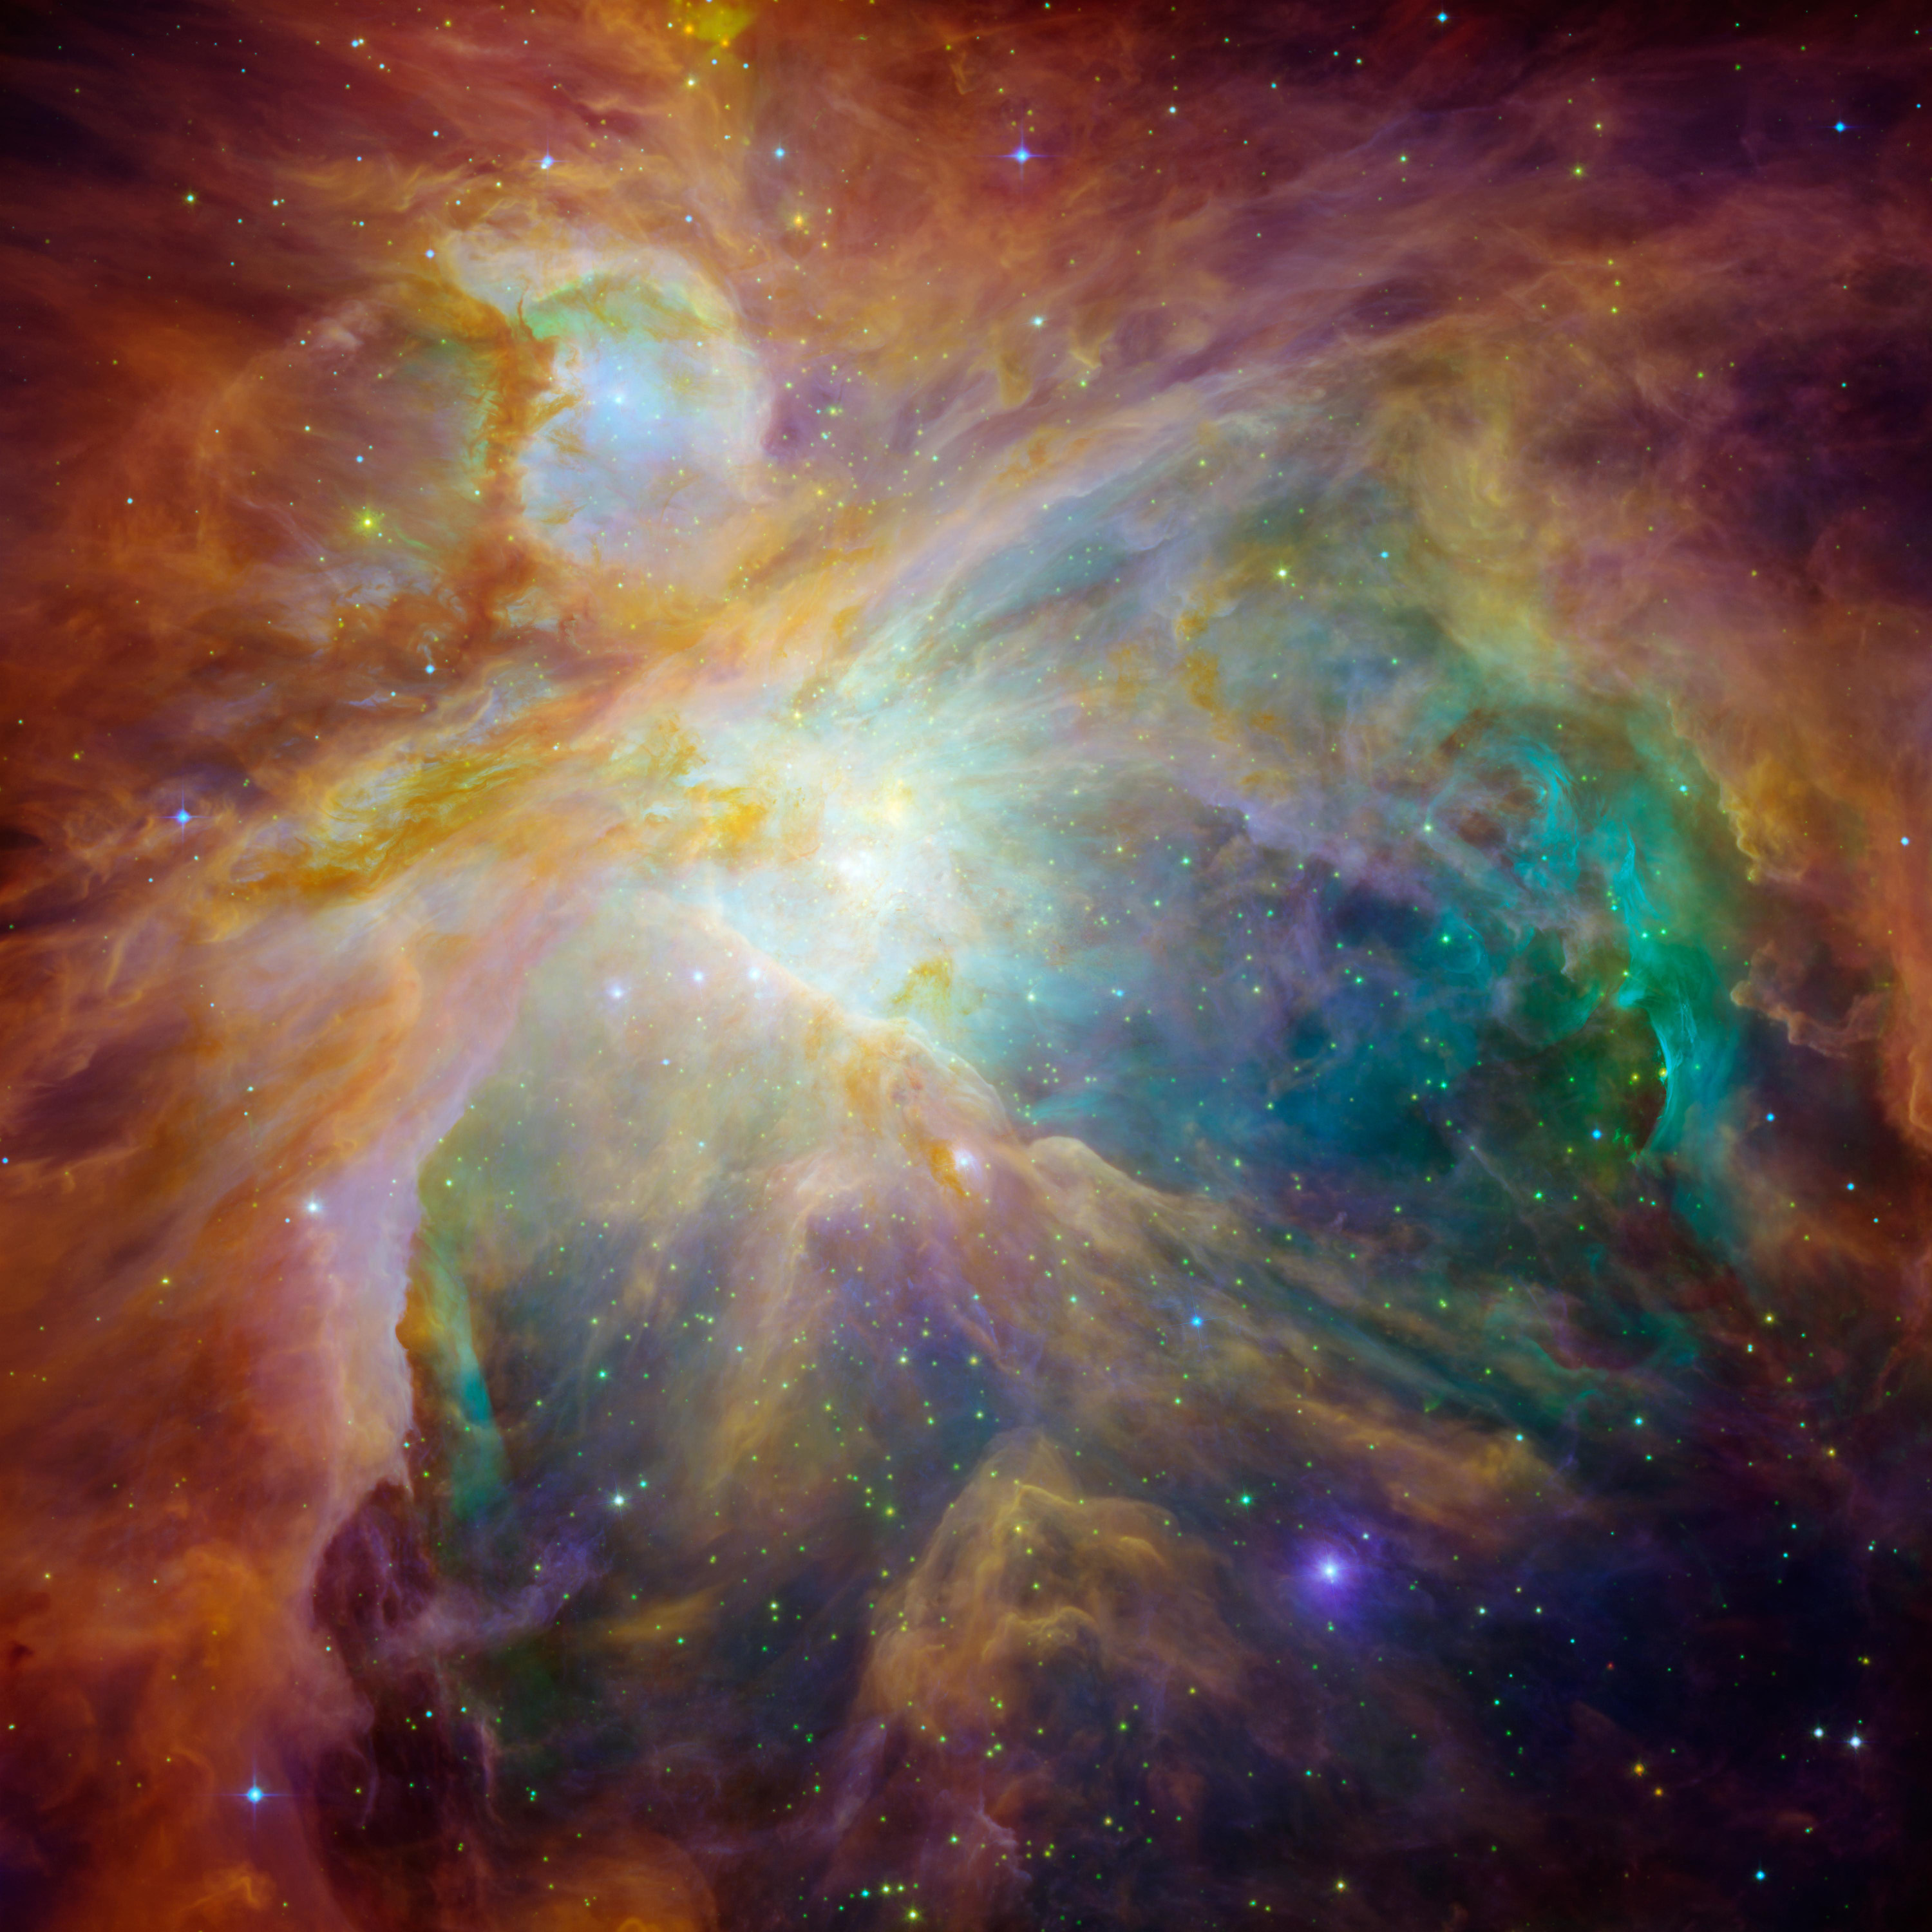
\includegraphics[width=\textwidth]{Figures/orion_nebula}
 \captionsetup{justification=justified,singlelinecheck=false,width=\linewidth}
 \decoRule
 \caption[The Orion Nebula]{The Orion Nebula: a false--color, composite image from NASA's Spitzer Space Telescope (SST) and Hubble Space Telescopes (HST).
			    The SST used its Infrared Array Camera (IRAC), while HST's Advanced Camera for Surveys (ACS) probed in the visible spectrum.
			    Amongst several others, the common H$\alpha$, SII and OIII filters were used to map the observations to rgb colors.\\
			    \textit{Image credit: NASA/JPL--Caltech/STScI}}
 \label{fig:Orion_nebula}
\end{figure}

% Description of the picture ----------------------------------------------------------------------------------------
The right side of the picture shows green and blue regions of heated, ionized gas intensely emitting ultraviolet radiation, evidence for sulfur and hydrogen.
In the left part there are darker clouds in yellow, orange and red color from infrared radiation, showing fewer stars due to the high column density of dust blocking all light below visible wavelengths.
The center shows a very massive, newly formed star cluster, identifiable as a bright yellow smudge, emitting radiation which erodes the region around it, while its stellar winds blow the gas even further away.
This extraordinarily massive cluster is even suspected to hold a black hole, roughly 200 times more massive than our Sun; see \citet{Orion_BH}.
\\[6pt]
%
% ISM ----------------------------------------------------------------------------------------
Molecular clouds are found in the interstellar medium (hereafter ISM), the material between star systems in galaxies.
The ISM is still quite mysterious and there is a considerable number of unsolved problems involving it, yet the physics of the ISM has been subject to research for a long time; see \citet{Draine, Unsolved_Problems}.
It is primarily composed of hydrogen, in atomic, ionized, and molecular form, usually denoted by HI, HII, and H$_{2}$, which leads to a separation into roughly three phases governed by the very different cooling mechanisms which are dominant for each kind.
Although the three--phase theory of the ISM was published over 35 years ago by \citet{ISM_3Phases}, it is still the prevailing model and hasn't been changed drastically since.
Each phase is thought to be in thermal pressure equilibrium, where heating and cooling rates are balanced.
Their equilibrium temperatures are around $10^{6}$ K, $10^{4}$ K, and $10$ K respectively, and their typical densities are $10^{-1}$ H/cc, $1$ H/cc, and $10^{3}$ H/cc.
\\[6pt]
%
% Numbers for MC ----------------------------------------------------------------------------------------
In the broad morphology of molecular clouds, some properties, like total mass, can vary widely and over several orders of magnitude.
Giant molecular clouds can have masses in the range of $10^{4}$--$10^{6}$~M$_{\odot}$ and stretch up to 200 pc in diameter; see \citet{GMC_Masses} and \citet{MC_Masses}.
The main constituent part of the clouds, as their name leads to presume, is molecular hydrogen H$_{2}$.
Typical temperatures in these clouds are around 10 K.
This low--temperature, high--density phase of the ISM is necessary in order to form dense enough regions to offset the balance between gravity and thermal pressure, thereby initiating gravitational collapse to form stars.
Higher temperatures would result in a thermal expansion and consequently in a reduction of the gas density.

% Observation ----------------------------------------------------------------------------------------
Even though the Orion Nebula can partially be seen on clear winter nights due to emission from ionization, most parts of molecular clouds are usually invisible to the naked eye.
The medium is much too cold to radiate in the visible spectrum.
Thus, in the exploration of molecular clouds radio and infrared astronomy is indispensable.
With measurements of radio emission from tracer molecules, such as CO, the structure of the gas clouds can be probed; see \citet{CO_tracing, Lada, Cham_cores_ALMA, Orion_cores}.

% Dust ----------------------------------------------------------------------------------------
Apart from gas, molecular clouds are also laced with dust, small solid grains which are able to absorb radiation below wavelengths of 1 $\mu$m quite efficiently.
The case of extremely high dust column densities blocking all the light from background stars defines another type of molecular cloud, the dark clouds.
Radiation from already formed, highly luminous star clusters in these clouds can excite the dust particles and raise their temperature to almost 100 K.
At the same time, these particles cool and prevent further climbing of their temperature by radiating in the infrared spectrum, which presents another possible method of observation.
\\[6pt]
%
% Turbulence ----------------------------------------------------------------------------------------
Molecular clouds are always highly turbulent, which is probably the main aspect of their beauty, but makes the life of a scientist so much harder; see \citet{Turbulence, KolmogorovC,KolmogorovB,KolmogorovA}.
Completely describing turbulence is a fairly difficult affair, so difficult in fact that it is still one of the unsolved problems in physics.
The origin of turbulence in the ISM is also still an open question.
Nevertheless, it is widely agreed upon that turbulence is a key factor in star formation; see \citet{Turbulence_key}.
Through turbulence energy is cascaded down the scale ladder, which makes star formation a multi--scale process.
How turbulent a cloud is, thus determines the dynamical scale on which the regulatory physics of star formation lie.
As long as turbulence is supersonic, which is observationally confirmed (\citealt{Turbulence_supersonic}), it represents the main contribution of opposing forces in the equilibrium with gravity.
However as turbulence dissipates on smaller scales due to shocks and viscosity, the cloud begins to fragment into clumps: compressed, denser regions, where the turbulent pressure is not strong enough and gravity takes hold.
This fragmentation process can happen repeatedly on different scale levels until gravitationally bound, homogeneous clumps remain.
These smallest clumps are called dense cores~\footnote{in some literatures also called molecular or in early stages starless cores} and ultimately collapse to protostars; usually they result in a whole set of protostars, called star cluster, but rarely in single stars.
\\[6pt]
%
% Importance of radiation ----------------------------------------------------------------------------------------
Once the star clusters have formed the demise of the molecular cloud is imminent.
One might be tempted to think that after the protostars have formed, they start to accrete the remaining gas in the cloud until all the material is consumed and only fully grown stars are left.
Observations and some theoretical considerations tell us another story: star formation is a very inefficient process in the sense that only a small fraction of the total cloud's mass is channeled into collapsing protostars, while most of it is blown outwards to repopulate the diffuse ISM; see \citet{SF_regulation, Padoan_PP}.
An enormous release of kinetic energy within a very short time span, such as a supernova explosion, could be responsible for the disruption of molecular clouds.
Observational estimates for the lifetime of molecular clouds however, are usually much shorter than the time, when the first supernova explosions occur; see \citet{MC_Masses, MC_supernovas}.
Currently the favored scenario which is thought to be responsible for the disruption of molecular clouds, is the ionizing radiation feedback from massive star clusters; see \citet{MC_disruption, Ionizing_disruption}.

\begin{figure}[ht]
 \centering
 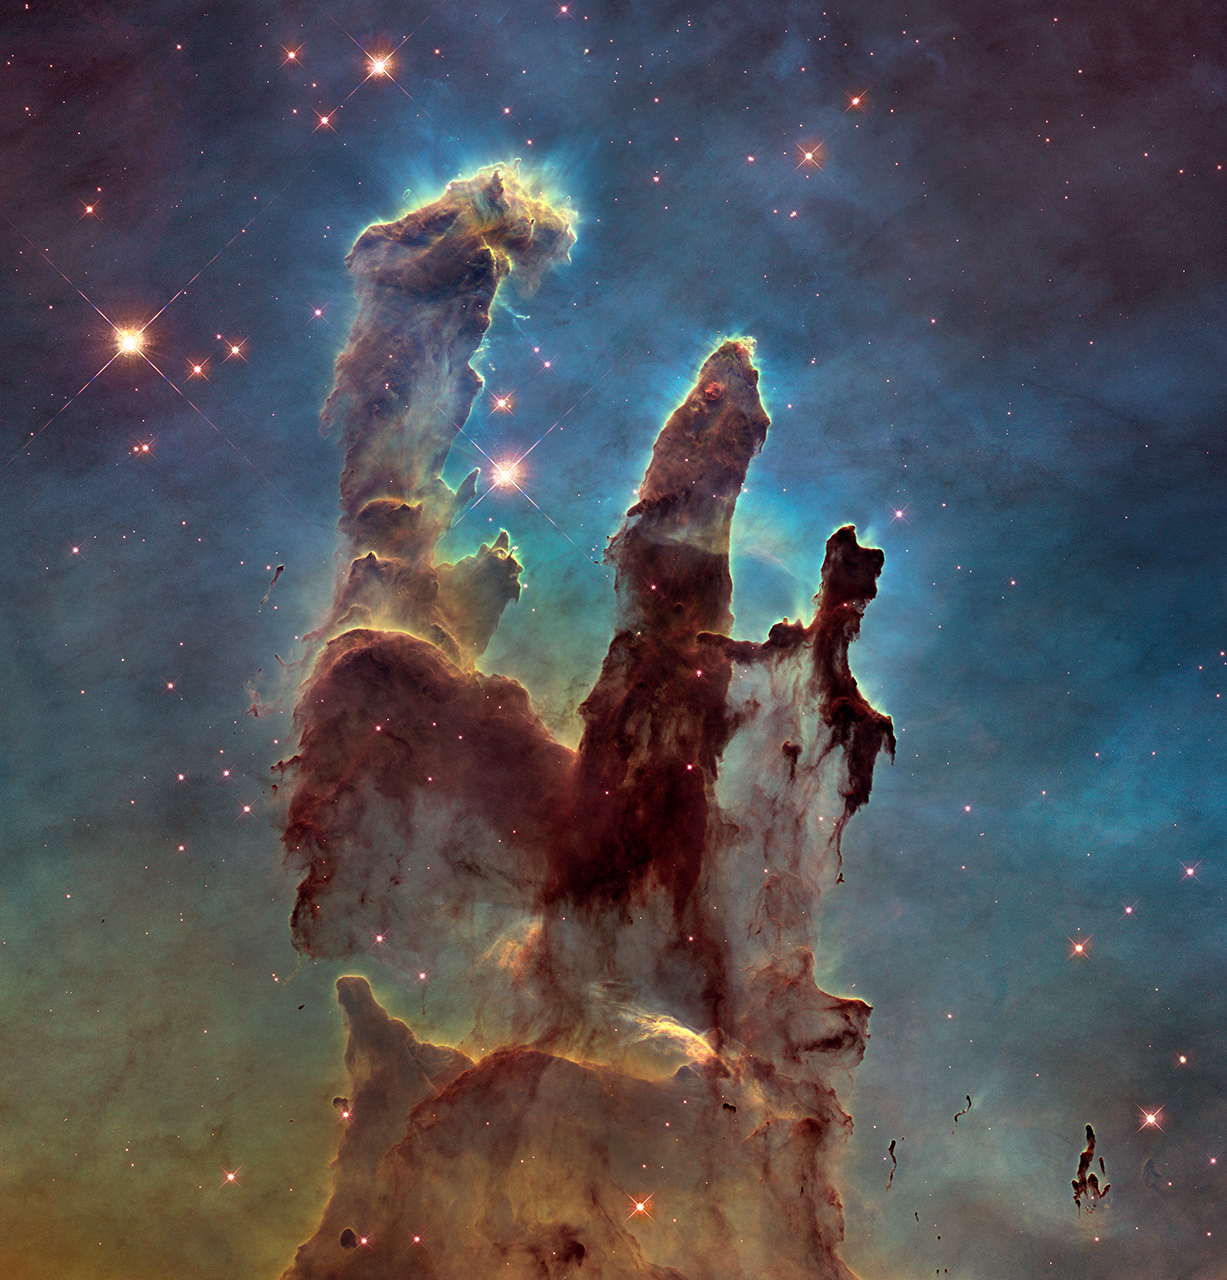
\includegraphics[width=\textwidth]{Figures/pillars_of_creation}
 \captionsetup{justification=justified,singlelinecheck=false,width=\linewidth}
 \decoRule
 \caption[Pillars of Creation]{A high-definition shot of NASA's iconic scenery, the 'Pillars of Creation', found in the Eagle nebula (M16).
          The name epitomizes the speculation that our own sun formed under a very similar nascent environment.
          All physical key processes of star formation are collected in a single picture:
          The pillar--like structure shows the turbulent nature of molecular clouds, while the gleaming tips of the towers show evidence of erosion by the hidden star cluster's radiation. \\
          \textit{Image credit: NASA, ESA/Hubble and the Hubble Heritage Team}
 }
 \label{fig:Pillars_of_creation}
\end{figure}

The influence and importance of radiative feedback is clearly shown in \figfigref{fig:Orion_nebula}{fig:Pillars_of_creation} both.
In \figref{fig:Orion_nebula} the region around the star cluster was already evacuated by its ionizing radiation, whereas in \figref{fig:Pillars_of_creation} the radiation just begun to erode the gas at the top of the pillars.

A standing goal of many computational astrophysicists is to reproduce the formation and evolution of whole galaxies and similar astronomical objects.
Over the years, a great deal of insight has been gained from hydrodynamical simulations, but there are still many open problems and a complete, physical simulation has yet to be run.
However these simulations also made it clear that radiation feedback has to be included and accurately modeled to make it one step further towards a realistic simulation.

% ----------------------------------------------------------------------------------------
\section{More and more questions}

After this short introductory overview on the birth places of stars, we will go into some important aspects of the very complex topic of star formation in more detail in the next few chapters.
To this date, the overall theory of the process of star formation is roughly outlined and in the star formation community to most parts accepted, the details are somewhat vague and debatable at times.
Some aspects have already been tested by numerical simulations --- a strong tool available to theoretical astrophysicists, when dealing with complex multi--physical scenarios ---, others have only now become possible to explore thanks to increasing computing power, and highly scalable and efficient astrophysical hydrodynamics codes.
\\[6pt]
%
% Personal learning process and structure ----------------------------------------------------------------------------------------
This thesis will be a recount of all the things I learned in the past year while working in computational astrophysics on the topic of star formation.
Thus, the following discussions will first cover the basics and impart analytical tools for processes involving hydrodynamical and radiative effects in astrophysics in general.
Due to a very limited starting knowledge in astrophysics when I began in this field of research, I had to ask very basic and at first glance maybe simple, but nonetheless important questions:
\\[-9pt]
\begin{itemize}
  \item Where and under what conditions do stars form? \\[3pt]
        Some answers to this question were outlined in this chapter; see \secref{sec:MolecularClouds}.
        Knowing where stars form, gives insights into the circumstances leading to star formation, which in turn determines the predominant physics involved.
        Once the driving forces are uncovered, the construction of physical models can commence, and raises subsequent question.\\[-9pt]

  \item How does a fluid, particularly molecular gas, move in a self--gravitational potential? \\[3pt]
        In the next \chapref{Chapter2}, \secref{sec:HydrodynamicEquations}, we will see idealized mathematical descriptions of the kinematics of fluids.
        These descriptions can be solved for equilibrium solutions, which give hints to possible configurations favorable for star formation and their instabilities; see \secref{subsec:Hydrostatic_equilibrium}. \\[-9pt]

  \item How does molecular gas collapse and fragment? \\[3pt]
        Behind this question lies importance for physics as well as for computational science.
        Fragmentation, or the lack thereof, can be the result of a multitude of physical processes.
        Investigating all of them is beyond the scope of this thesis.
        Thus, this thesis lays the focus on a single specific effect, which is also part of the next question.
        Of special relevance for fragmentation are mass, length and time scales and conditions for gravitational stability of gas.
        These are also of particular importance for the resolution requirements of (sub--)grid models in computer simulations.
        \secref{subsec:Instabilities} will explain the relevant physics of gravitational collapse and gas fragmentation.
        The description of some of the grid models and their specific requirements are discussed in \secref{sec:AMR}. \\[-9pt]

  \item How does an initially rotating sphere evolve into a star forming core? \\[3pt]
        This question addresses the issue of initial conditions and simplification of given problems.
        The choice of initial conditions depends on the part of the problem one wants to focus on.
        When setting up a simulation for instance, there are important aspects one has to consider in order to realistically reproduce the problem or process.
        What cases are even possible to simulate? Where can simplifications be made without the loss of physics in focus?
        \secref{subsec:Larson_cores}, explains the simplified model which still considers the basic physics involved in star formation.
        \secref{subsec:Initial_conditions}, describes how the initial conditions for these models were numerically implemented. \\[-9pt]

  \item How does radiation and other physical modes influence molecular gas? \\[3pt]
        The second part of the next chapter, \secref{sec:RadiativeTransfer}, introduces the basic theory how radiation interacts with matter.
        Knowing in detail how radiation affects the gas (see \secref{subsec:Coupling_to_HD}) during a certain phase in prestellar collapse could explain some discrepancies between simulations and observations of young star clusters. \\[-6pt]
\end{itemize}

These questions represent my thinking and learning process and should give a common thread through star formation theory.
This thesis consists of part theoretical physics which is structured through the questions above, and part computational science which is discussed in \chapref{Chapter3}.
Computational astrophysicists have already realized that the theory of star formation and radiation hydrodynamics are intertwined, but including radiation in hydrodynamics simulations requires much more computational resources, which is why one often relied on computationally cheaper, but inexact sub--grid models.
To date simulations including both are considered state--of--the--art.
Methods working towards this objective are discussed in \secref{sec:Godunov}, (\ref{sec:MUSCL}), (\ref{sec:Source_terms}) and (\ref{sec:AMR}).

In \chapref{Chapter2} and (\ref{Chapter3}) I gather and present the necessary common knowledge in order to be able to investigate star formation with computer simulations.
These simulations and their results are presented and discussed in \chapref{Chapter4}.
%TODO
The main goal of this thesis was to test the numerical model for radiation hydrodynamics (see \chapref{Chapter4}), specifically the infrared radiation treatment for star formation, which was already implemented in the adaptive mesh refinement code RAMSES, mentioned in \secref{sec:RAMSES}.
The final result of this test will be the simulation of an entire molecular cloud; see \secref{sec:MC}.
